% ============================================================
%  Chapter 1: Introduction
% ============================================================

\chapter{Introduction}

% ============================================================
\section{Project Overview}
% ============================================================

Two misconfigurations, neither exotic, combine to produce full host compromise
from a single HTTP request. No kernel exploits are involved. No CVEs need to be
present. The attack chain demonstrated in this project requires only two
operator-level decisions that are depressingly common in real deployments:
unsanitised user input passed to a shell via \texttt{os.popen()}, and the host
Docker socket bind-mounted into a running container.

The application under test is \textbf{NetDiag}, a fictional internal network
diagnostic tool built on Flask. NetDiag is designed to look plausible --- it
carries an \textit{INTERNAL USE ONLY} badge, presents a clean web interface, and
exposes a single utility endpoint that pings a user-supplied hostname. That
endpoint, \texttt{/ping}, executes the following on the server:

\begin{verbatim}
os.popen("ping -c 3 " + host)
\end{verbatim}

A semicolon in \texttt{host} terminates the \texttt{ping} command. Every
character that follows runs in the same shell, as the same user --- root inside
the container. The container itself has no \texttt{USER} directive and was
started with \texttt{-v /var/run/docker.sock:/var/run/docker.sock} mounted into
it. These two decisions are individually bad. Together they are catastrophic.

The full attack chain proceeds as follows. The attacker, operating from a
separate machine, sends a crafted HTTP request to the \texttt{/ping} route. The
injected payload opens a reverse shell back to the attacker. From inside that
shell the attacker communicates with the Docker daemon over the mounted Unix
socket, uses the Docker API to pull and run a new privileged container with the
host root filesystem mounted at \texttt{/mnt/host}, and writes a file directly
to the host filesystem --- achieving a complete container escape without ever
touching a kernel vulnerability.

\begin{figure}[h]
\centering
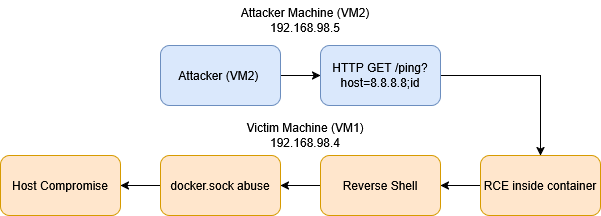
\includegraphics[width=\textwidth]{images/attack_chain.png}
% DIAGRAM 1.1 --- Attack Chain Overview
% Horizontal left-to-right flow with 5 nodes across two swim lanes.
% Swim lane 1 (VM2 -- Attacker): Attacker (VM2) -> HTTP GET /ping?host=8.8.8.8;id
% Swim lane 2 (VM1 -- Victim): RCE as root in container -> Reverse Shell ->
%   docker.sock abuse -> Host Compromise (VM1)
% Each arrow labelled with its mechanism:
%   command injection | bash TCP redirect | Docker API call
\caption{Attack Chain Overview --- VM2 to Host Compromise on VM1}
\label{fig:attack-chain}
\end{figure}

The lab uses two virtual machines. \textbf{VM1} (\texttt{192.168.98.4}) is the
victim; it runs the Docker daemon and hosts the NetDiag container. \textbf{VM2}
(\texttt{192.168.98.5}) is the attacker; it sends the exploit request and
receives the reverse shell. Both machines run Kali Linux on a VirtualBox NAT
Network, giving them mutual reachability without exposure to the public internet.

Three scripts accompany this project. \texttt{setup.sh} runs on VM1 and builds
the NetDiag image, removes any previous instance, and starts the container with
the exact flags that create the vulnerable configuration. \texttt{attack.sh}
runs on VM2 and walks through the full exploitation chain step by step, with
output annotated at each stage. \texttt{detect.sh} runs on VM1 after the attack
and demonstrates post-incident detection using \texttt{docker inspect},
\texttt{auditd}, and \texttt{lsof}.

% ============================================================
\section{Objectives}
% ============================================================

Four concrete objectives drive this project, each with a specific technical
end-state rather than a generic learning outcome.

\subsection{Demonstrate the Attack Chain End to End}

The primary objective is to show, reproducibly, that two common
misconfigurations combine to produce full host compromise. The specific end
state is a file written to \texttt{/tmp/escaped.txt} on the VM1 host
filesystem, created from inside the NetDiag container, confirming that the
attacker has escaped the container boundary entirely.

\subsection{Explain the OS-Level Mechanics}

Linux namespaces isolate the container at the PID, network, mount, and UTS
level. That isolation does not protect against this attack. The Docker socket is
a Unix domain socket owned by the Docker daemon, which runs on the host outside
any container namespace. Bind-mounting it into the container gives the container
a direct channel to that daemon. Because the container process runs as root with
a full capability set --- no \texttt{USER} directive drops privileges, no
\texttt{--cap-drop} removes capabilities at runtime --- it can send arbitrary
commands to the daemon, including requests to spawn new containers with
unrestricted host filesystem access. Namespace isolation is not a substitute for
capability restriction when a privileged communication channel is deliberately
handed to the contained process.

\subsection{Build and Document a Working Detection Toolkit}

Detection does not require a commercial SIEM or a dedicated security appliance.
The toolkit documented in this project uses tools available on any standard
Linux host:

\begin{itemize}
  \item \texttt{docker inspect} --- audits container mount configuration before
    or after an incident, revealing any bind-mount of
    \texttt{/var/run/docker.sock}.
  \item \texttt{auditd} with a \texttt{-w} watch rule on
    \texttt{/var/run/docker.sock} --- writes a kernel audit event every time the
    socket is opened, providing a timestamped record of access.
  \item \texttt{lsof} --- identifies in real time which processes hold the
    socket file descriptor open, useful during a live incident.
  \item \textbf{Falco} --- referenced as the production-grade alternative; a
    kernel-level eBPF/syscall monitor that can alert on socket access, container
    escape indicators, and anomalous Docker API calls without requiring auditd
    configuration.
\end{itemize}

\subsection{Document Concrete Mitigations}

Mitigation requires two targeted fixes. At the application layer, replacing

\begin{verbatim}
os.popen("ping -c 3 " + host)
\end{verbatim}

\noindent with

\begin{verbatim}
subprocess.run(['ping', '-c', '3', host], capture_output=True)
\end{verbatim}

removes the shell entirely. The user-supplied value is passed as a list element
to \texttt{execve} and is never interpreted by a shell parser, so no injected
metacharacter can break command context. At the infrastructure layer, removing
\texttt{-v /var/run/docker.sock:/var/run/docker.sock} from the \texttt{docker
run} invocation closes the escape route even if command injection remains
present. Rootless Docker, Podman, and Docker Socket Proxy are documented as
architectural alternatives for deployments that genuinely require socket access
from within a container.

% ============================================================
\section{Lab Environment Summary}
% ============================================================

\subsection{Physical Setup}

The lab consists of two Kali Linux virtual machines running under VirtualBox in
NAT Network mode. NAT Network gives each VM a private IP address and routes
traffic between them through a VirtualBox virtual switch; neither machine has a
route to the public internet, which is not required for any part of this
demonstration. VM1 is assigned \texttt{192.168.98.4} and acts as the victim. VM2
is assigned \texttt{192.168.98.5} and acts as the attacker. The assigned
addresses can be verified on either machine with \texttt{ip a}, which queries
the kernel's interface table and prints the IPv4 and IPv6 addresses bound to
each network interface.

\subsection{VM1 --- Victim Machine}

VM1 runs the Docker daemon (\texttt{dockerd}) as a root-owned system service.
\texttt{dockerd} itself runs as root on the host and owns the Unix socket at
\texttt{/var/run/docker.sock}, created with mode \texttt{660} and group
\texttt{docker} by default. The NetDiag container is started by
\texttt{setup.sh} with the following command:

\begin{verbatim}
docker run -d \
  -p 5000:5000 \
  -v /var/run/docker.sock:/var/run/docker.sock \
  --name netdiag-app \
  netdiag
\end{verbatim}

Each flag has a specific OS-level effect. \texttt{-d} runs the container in
detached mode, disconnecting it from the terminal's standard input and placing
it under daemon supervision. \texttt{-p 5000:5000} installs an iptables DNAT
rule on the host that rewrites packets arriving at host port 5000 and forwards
them to the container's port 5000 via the \texttt{docker0} bridge interface.
\texttt{-v /var/run/docker.sock:/var/run/docker.sock} creates a bind mount: the
kernel maps the host inode for the socket file directly into the container's
mount namespace at the same path, so any process inside the container that opens
that path is in fact opening the host socket. The \texttt{--name netdiag-app}
flag assigns a human-readable name used by \texttt{detect.sh} when calling
\texttt{docker inspect}.

The container process runs as root. The Dockerfile contains no \texttt{USER}
directive, and no \texttt{--user} flag is passed at runtime. Inside the
container, the Flask application is bound to \texttt{0.0.0.0:5000}, making it
reachable on all container interfaces and, via the port mapping, on all host
interfaces --- including the one facing VM2.

\subsection{VM2 --- Attacker Machine}

VM2 uses no tools beyond those shipped with Kali Linux: \texttt{curl} for HTTP
requests and \texttt{nc} (netcat) for the reverse shell listener. No
vulnerability scanner, no exploit framework, and no prior access to the NetDiag
source code is required. The vulnerability is discovered through direct
interaction with the \texttt{/ping} endpoint: the response timing and content
change when shell metacharacters are appended to the \texttt{host} parameter,
confirming that input reaches the shell unfiltered.

\subsection{Network Topology}

\begin{figure}[h]
\centering
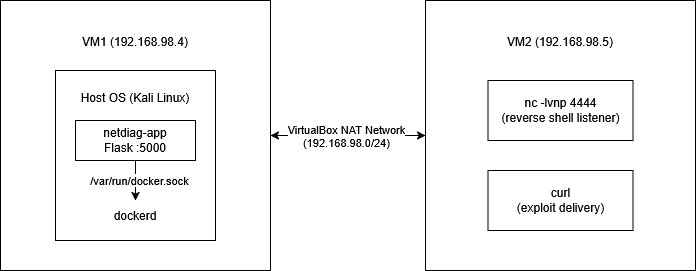
\includegraphics[width=\textwidth]{images/lab_network_topology.png}
% DIAGRAM 1.2 --- Lab Network Topology
% Two side-by-side boxes: VM1 (192.168.98.4) and VM2 (192.168.98.5).
% Inside VM1: Host OS (Kali) box containing a nested Docker container box
%   labelled "netdiag-app (Flask :5000)".
% A line labelled "/var/run/docker.sock" connects the container box to a
%   "dockerd" label on the host OS layer.
% An arrow labelled "port 5000 (iptables DNAT)" crosses the VM1 boundary.
% A bidirectional arrow between the two VM boxes labelled
%   "VirtualBox NAT Network (192.168.98.0/24)".
% Inside VM2: labels "nc -lvnp 4444 (reverse shell listener)"
%   and "curl (exploit delivery)".
\caption{Lab Network Topology --- VirtualBox NAT Network}
\label{fig:lab-topology}
\end{figure}

\subsection{Software Versions}

The following versions were used during development and testing. Confirm each
value on the live VMs before final submission.

\begin{itemize}
  \item Kali Linux: \textit{(fill in from \texttt{uname -a} on VM1)}
  \item Docker Engine: \textit{(fill in from \texttt{docker --version} on VM1)}
  \item Python inside the container: \textit{(fill in from \texttt{python3 --version} inside the container)}
  \item Flask: \textit{(fill in from \texttt{pip show flask} inside the container)}
\end{itemize}

% ============================================================
\section{Scope and Limitations}
% ============================================================

\subsection{What Is In Scope}

This project addresses the specific two-vulnerability chain: command injection
via unsanitised shell execution combined with the \texttt{docker.sock} bind
mount. Detection methodology uses tools available on a default Kali Linux
installation supplemented by \texttt{auditd}. Mitigation is addressed at two
levels: the application source code and the container runtime invocation.
OS-level explanation of why PID and mount namespace isolation does not
neutralise this attack is included in Chapter~2.

\subsection{What Is Explicitly Out of Scope}

\begin{itemize}
  \item \textbf{Kernel exploits} --- Dirty Pipe (CVE-2022-0847), Dirty COW
    (CVE-2016-5195), and runc CVEs (CVE-2019-5736) are not used and are not
    needed. This is deliberate: misconfiguration alone, without any unpatched
    CVE, is sufficient for full host compromise.
  \item \textbf{Container runtime CVEs} --- No patching is required on VM1. The
    vulnerable state is produced entirely by configuration choices, not by
    software defects in Docker or the Linux kernel.
  \item \textbf{Privilege escalation on VM2} --- The attacker operates from a
    standard user session on Kali. No local privilege escalation on the attacker
    machine is required or demonstrated.
  \item \textbf{Network-layer attacks} --- ARP spoofing, MITM interception, and
    similar techniques are not used. The attacker reaches the application
    directly over HTTP using the known IP address of VM1.
\end{itemize}

\subsection{Limitations of the Demo Environment}

The VirtualBox NAT Network does not represent a production network. In a real
deployment, a Flask application would typically sit behind a reverse proxy such
as nginx or Caddy, which would terminate TLS, apply rate limiting, and not
expose the application port directly to external traffic. The direct exposure of
port 5000 in this lab simplifies the demonstration but overstates the ease of
initial access in hardened environments.

The Kali base image used inside the container includes many pre-installed tools.
A minimal Alpine or Debian Slim base would require installing the Docker CLI
package before the escape step, which would add latency but would not change the
fundamental technique.

The \texttt{setup.sh} script calls \texttt{docker rm -f netdiag-app} before
each run, destroying the previous container and its filesystem overlay. In a
real incident the container filesystem would remain intact after the escape and
would preserve forensic artifacts: shell history, dropped binaries, and any
files created by the attacker before pivoting to the host.

\subsection{What the Demo Proves}

Two conclusions follow directly from the demonstration. First, operator-level
configuration decisions --- mounting the Docker socket and omitting a non-root
user directive --- carry more exploitability risk than most individual
application vulnerabilities in isolation. A perfectly hardened application
cannot protect itself if the container runtime hands it a direct channel to the
host. Second, detection is tractable without expensive tooling: \texttt{auditd},
\texttt{docker inspect}, and \texttt{lsof} are available everywhere, cost
nothing, and produce actionable evidence.

% ============================================================
\section{Ethical Disclaimer}
% ============================================================

This project was conducted entirely within a closed VirtualBox environment with
no external network connectivity. No real systems, services, or data were
targeted at any point. The NetDiag application was written specifically for this
project and contains an intentional vulnerability; it is not derived from any
real production codebase.

The techniques demonstrated are documented in public security research: the OWASP
Testing Guide covers OS command injection; Docker's own security documentation
explicitly warns against mounting the Docker socket; the MITRE ATT\&CK framework
catalogues the relevant techniques as T1610 (Deploy Container) and T1611 (Escape
to Host). These techniques appear in offensive security training curricula ---
OSCP, CEH, eJPT --- precisely so that defenders understand what they are
protecting against. Any reproduction of this work must be performed in an
isolated lab environment only.

% ============================================================
%  Chapter 1 Summary
% ============================================================

\vspace{1em}
\noindent\rule{\textwidth}{0.4pt}
\vspace{0.5em}

\noindent\textbf{Chapter 1 Quick Reference}

\begin{itemize}
  \item Two Kali Linux VMs on a VirtualBox NAT Network; one vulnerable Flask
    application; one Docker socket misconfiguration.
  \item Attack chain: Command Injection $\rightarrow$ Reverse Shell
    $\rightarrow$ \texttt{docker.sock} abuse $\rightarrow$ Host Compromise.
  \item No kernel exploits. No CVEs. Misconfiguration alone is sufficient.
  \item Detection is possible with \texttt{auditd}, \texttt{docker inspect}, and
    \texttt{lsof}. Mitigation requires two targeted fixes: one in application
    code, one in the container run command.
\end{itemize}

\noindent\rule{\textwidth}{0.4pt}